\chapter{INTRODUCTION} \label{chap:introduction}
    %\doublespacing
    \minitoc
    \emph{Abstract of chapter \ref{chap:introduction}}
    
    \section{Introduction} \label{introduction:introduction}
        
        \subsection{X-ray Astronomy} \label{introduction:introduction:x-ray-astro}
        	Today X-ray astronomy is recognized as a mature and important branch of astronomy. Observations made in the X-ray window enable us to understand many high-energy events in the Milky Way and other galaxies. The physics of such events have improved our understanding of stellar and galactic evolution. Since our atmosphere is opaque to X-rays, observations in this band need to be carried out from outer space. Starting with the Uhuru in 1970, a series of satellites with X-ray telescopes have been launched, leading to the discovery of new and exotic classes of X-ray sources.
        	
        	In X-ray astronomy, the principle mode of measurement is to detect individual photons so as to determine its \emph{arrival direction}, \emph{energy}, \emph{time of arrival} and the \emph{polarization angle} \cite{overviewXrays}. The refinement of the instruments on board space-based X-ray observatories have led to greater spectral resolution of the observed X-ray objects. Initially, X-ray detectors were proportional counters and scintillation counters. The introduction of focusing and imaging X-ray optics, the Wolter telescope, together with imaging detectors in the focal plane allowed the capture of 2D X-ray imagery. Today, the pioneering X-ray satellites, namely Chandra and XMM-Newton, have actively cooled pixelized solid-state detectors as their standard focal plane detector, providing higher energy resolution and wider energy range than proportional counters.In addition to imaging telescopes, high-resolution grating spectrometers, which have very high spectral resolution and large throughput, are also used in the Chandra and XMM-Newton missions \cite{paragb2017rev}.
        
        \subsection{Supersoft X-ray Sources} \label{introduction:introduction:sss}
        	Luminous supersoft X-ray sources (SSS) were first identified as an important new class of intrinsically bright X-ray sources by Tr{\"u}mper \emph{et al.}\cite{trumper91}, Greiner \emph{et al.}\cite{greiner91} and Kahabka \emph{et al.}\cite{kahabka06}. SSS are now classified as sources with X-ray luminosities of the order of the Eddington limit ($\sim 10^{38}$ erg s$^{-1}$), and with extremely soft spectra peaking in the energy range 15--80 eV -- corresponding to a blackbody temperature of $\sim\,$300,000--500,000 K (Kababka \emph{et al.})\cite{kahabka97}.
        	
        	The first SSS were observed by the low-resolution proportional counters on board the Einstein and ROSAT satellites. Presently, high-resolution X-ray spectra have been obtained by Chandra and XMM-Newton for a number of SSS, some of the most remarkable ones include RX J0925.7-4758 \cite{bearda2002,motch2002}, CAL 83 \cite{lanz2005}, CAL 87 \cite{orio2004} and RX J0019.8+2156 \cite{schwarz2004}.
        	
        	The currently accepted model for luminous SSS is that, with a few exceptions, these sources are accreting white dwarfs (WDs) within a binary system, \emph{which are burning hydrogen within their envelopes in a steady or intermittent manner} \cite{vandenHeuvel92}.
    
    \section{Background} \label{introduction:background}
        From being a mere curio, today the study of SSS is regarded as being crucial to the understanding of the evolution of X-ray binaries. A large proportion of the SSS discovered so far are transient. Supersoft transients seem to be classical and symbiotic novae having a supersoft phase and also systems with no known nova outburst but exhibit supersoft X-ray ``on'' and ``off'' states. Although the evolution of type Ia supernovae (SN Ia) has not been fully solved as yet, keeping in mind their calculated numbers and birth rates, merging double degerate white dwarfs and CBSS are considered to be the two most promising progenitor candidates for SN Ia. The SSS spectra for several sources obtained with high-resolution grating spectrometers reveal the dominance of several spectral features, including P Cygni profiles. Obtaining a proper fit for such spectra has been challenging so far, but crucial in order to be able to derive the parameters of the SSS under study.
    
    \section{Current Status} \label{introduction:current_status}
        A brief summary of the current literature concerning the study of observational data from SSS is discussed in the current section.
        
        \subsection{Supersoft X-ray Sources as a New Class of Luminous X-ray Sources} \label{introduction:current_status:new-class}
        	The limited spectral range and resolution of the Einstein satellite did not allow the first four luminous SSS discovered by it to be recognised as a separate class \cite{long81,seward81}. It was due to the enhanced spectral range and resolution of the ROSAT that SSS were later distinguished as a class of sources different from classical strong-point X-ray sources, such as accreting neutron stars or black holes in binaries. SSS have been observed to have a distinctive peak around 15--80 eV, corresponding to blackbody temperatures that are around 2 orders of magnitude lower than that of classical strong point X-ray sources.
        	
        \subsection{Currently Accepted Model for SSS} \label{introduction:current_status:SSS-model}
        	If the luminosity and effective temperature of a star are known, using the \emph{Stefan-Boltzmann's law}, one can derive its radius as follows
        	\begin{equation} \label{SSS-model:stef-boltz}
        		L=4\pi R^2\sigma T^4
        	\end{equation}
        	thereby yielding
        	\begin{equation} \label{SSS-model:star-radius}
        		R=9\times 10^8(L_{37.5})^{1/2}(T_e/40\,\mathrm{eV})^{-2}\,\mathrm{cm,}
        	\end{equation}
        	where $L_{37.5}$ is the X-ray luminosity in units of $10^{37.5}$ erg/s, and $T_e$ is the effective temperature in electron volts.
        	
        	Using the characteristic values for SSS, namely $L_{37.5}=1$ and $T_e=40$ in equation (\ref{SSS-model:star-radius}), we obtain that the radius of the emitting object is around 9000 km, \emph{which is similar to that of a white dwarf}. Analogous to accreting neutron stars and black holes in classical X-ray binaries, this suggests that supersoft X-rays are generated by the accretion of matter onto a white dwarf.
        	
        	Van den Heuvel argued that for white dwarf masses in the range $0.7-1.4\,M_{\odot}$ and with mass accretion rates in the range $\sim 1-5\times 10^{-7}\,M_{\odot}\,yr^{-1}$, supersoft X-rays are produced \cite{vandenHeuvel92} (here $M_{\odot}$ refers to solar mass). In such models, it is assumed that the mass-accretor is the white dwarf, and the companion star is a main-sequence star with a mass in the range $1.4-1.5\,M_{\odot}$ or a post-main-sequence star with a mass in the range $1.5-2\,M_{\odot}$. Theoretically, the mass-transfer rates by Roche-lobe overflow for these companion masses were derived to be $\sim 10^{-7}\,M_{\odot}\,yr^{-1}$ and $\sim 4 \times 10^{-7}\,M_{\odot}\,yr^{-1}$ respectively. The X-ray lifetimes were determined to be $\sim 10^{7}$ years.
        	
        	Nomoto showed that there are 3 possible regimes of nuclear burning in the surface layers of a white dwarf (depicted in Figure \ref{fig:regimes-wd}), depending on the accretion rate and the white dwarf mass \cite{nomoto82}. These regimes are summarized as follows, for a white dwarf with solar mass:
        	
        	\begin{figure}[h!]
        		\begin{center}
        			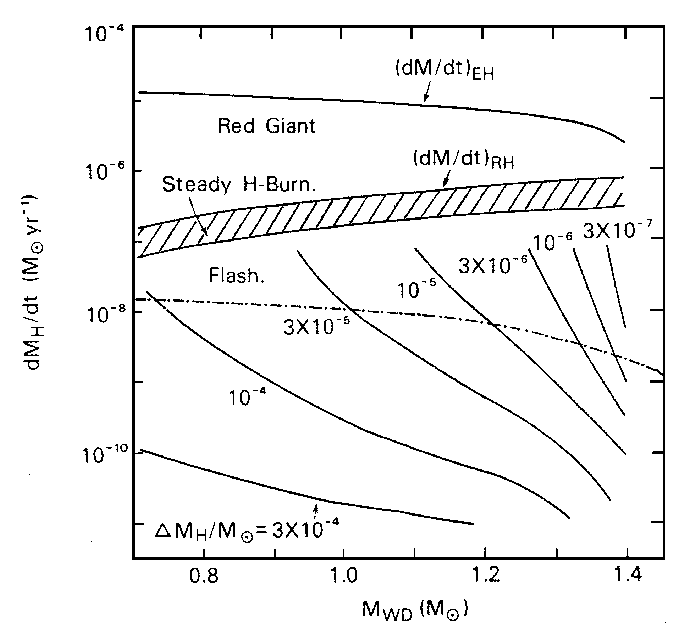
\includegraphics[scale=1.2]{sss-regimes.eps}
        			\caption{The regimes of nuclear burning in the surface layers of a white dwarf \cite{nomoto82}}
        			\label{fig:regimes-wd}
        		\end{center}
        	\end{figure}
        	
        	\begin{enumerate}
				\item For mass accretion rate in the narrow range $1-4\times 10^{-7}\,M_{\odot}\,yr^{-1}$, the accreted hydrogen burns steadily, without any significant radius expansion of the white dwarf.
				\item For mass accretion rates below the range of steady burning, the accreted matter burns in flashes, i.e. intermittently. With decreasing accretion rates, the frequency of the flashes decreases and the flashes themselves become more violent.
				\item For mass accretion rates above the range of steady burning, the radius expands to red giant dimensions, and the matter continues to burn steadily within a thin shell around the white dwarf. This, incidentally, corresponds to the growth rate of the degenerate core in red giant stars due to the hydrogen shell burning.
			\end{enumerate}
			
			Calculations by Hachisu \emph{et al.} show that when the mass accretion rates are very high, much beyond the steady-burning range, a stellar wind solution replaces the static envelope solution \cite{hachisu96}. This stellar wind flows out from the white dwarfs at high speeds ($\sim 5000$ km/s). Because this stellar wind is opaque to soft X-rays, such radiation do not escape. So long the accretion rate remains within steady-burning range, the white dwarf will be observed as a steady, luminous SSS. According to Hachisu \emph{et al.}, the white dwarf steadily burns hydrogen and accretes helium, thereby increasing its mass up to $1.38\,M_{\odot}$ and then explode as an SN Ia. Therefore, there is a strong suggestion that \emph{SSS could be a possible progenitor for SN Ia}.
		
		\subsection{Possible Companions to a White Dwarf in SSS} \label{introduction:current_status:wd-companions}
			\subsubsection{Near main-sequence stars more massive than WDs}
				The simplest binary configuration that can become a luminous SSS comprises of a white dwarf with a companion star whose mass is larger than about $1.3\,M_{\odot}$ and has a radiative envelope. In such a system, once the donor star overflows its \emph{Roche lobe}, mass transfer to the white dwarf starts, causing its orbit to shrink. The donor becomes thermally unstable and it will continue transferring mass until it becomes less massive of the two and further mass transfer leads to the orbit expansion (Paczynski) \cite{paczynski71}. Such systems are called \emph{close-binary supersoft sources} (CBSS). Nine CBSS have been identified by Greiner \cite{greiner2000catalog,greiner2000catalogOnline}.
				
			\subsubsection{Symbiotic systems}
				Sion \emph{et al.}\cite{sion94} first showed that a system consisting a red-giant star and a white dwarf is another class of binary systems which can sustain the mass accretion rates necessary for producing supersoft X-rays. Two types of red-giant companions may be expected, providing different modes of mass-transfer.
				
				\begin{enumerate}
					\item $1\,M_{\odot}$ red-giant, less massive than the white dwarf. Such a companion overflows its Roche lobe with an orbital period of at least 125 days. The red-giant has a degenerate He core, and its nuclear evolution drives the mass transfer.
					\item The red-giant is on the aymptotic giant branch (AGB) and is not filling its Roche lobe, however there is a very strong stellar wind. With mass loss rates from the AGB of the order $10^{-5}\,M_{\odot}\,yr^{-1}$ and stellar wind velocities of around 30 km/s, the aggregate accretion rate can become as large as of the order $10^{-7}\,M_{\odot}\,yr^{-1}$ on a white dwarf, which is sufficient to create a luminous SSS.
				\end{enumerate}
		
		\newpage
		\subsection{Classification Scheme for SSS} \label{introduction:current_status:sss-classification}
			As per di Stefano \emph{et al.} \cite{distefano96}, binary systems that may appear as luminous SSS may be classified as follows:
			
			\begin{center}
				\begin{table}[h!]
					\label{tab:SSS-class}
					\caption{Classification of binary systems that may manifest as SSS}
					\begin{tabulary}{\textwidth}{CCCCC}
						\hline
						\small{\textbf{[A] System Type}} & \small{\textbf{[B] Mass Transfer Mechanism}} & \small{\textbf{[C] Mass Accretion Rate $\boldsymbol{\dot{M}}$ ($\boldsymbol{M_{\odot}}$ yr$^{-1}$)}} & \small{\textbf{[D] Orbital Period $\boldsymbol{P}_\text{\textbf{orb}}$ (days)}} & \small{\textbf{[E] Steady or Recurrent}}\\
						\hline
						\small{CVs} & \small{mb and/or gr} & \small{$\lesssim 10^{-8}$} & \small{$\lesssim 0.2$} & \small{R}\\
						\hline
						\small{CBSSs} & \small{thermal time scale readjustment of donor} & \small{$\gtrsim 10^{-7}$} & \small{$\sim 0.2-3.0$} & \small{S}\\
						\small{} & \small{} & \small{$\lesssim 10^{-7}$} & \small{$\sim 0.2-\mathscr{O}(10^2)$} & \small{R}\\
						\hline
						\small{WBSSs} & \small{nuclear evolution of donor} & \small{$\gtrsim 10^{-7}$} & \small{$\sim 3.0-\mathscr{O}(10^2)$} & \small{S}\\
						\small{} & \small{} & \small{$\lesssim 10^{-7}$} & \small{$\sim 3.0-\mathscr{O}(10^2)$} & \small{R}\\
						\hline
						\small{Symbiotics (Wind-driven)} & \small{stellar winds from evolved donor} & \small{$\gtrsim 10^{-7}$} & \small{$\mathscr{O}(10^2)$} & \small{S}\\
						\small{} & \small{} & \small{$\lesssim 10^{-7}$} & \small{$\mathscr{O}(10^2)$} & \small{R}\\
						\hline
					\end{tabulary}
				\end{table}
			\end{center}
			
			In the table above, [A] only those systems are considered in which H-rich material is accreting on the surface of a C-O white dwarf. Here CV = cataclysmic variable, CBSS = close-binary supersoft source and WBSS = wide-binary supersoft source. [B] Two prominent mass transfer mechanisms are mb = magnetic braking and gr = gravitational radiation. [C] $\dot{M}$ is the mass accretion rate on the surface layers of the white dwarf. [D] $P_\text{orb}$ refers to the orbital period of the binary. [D] When $\dot{M}$ is in the correct range (about $\gtrsim 10^{-7}\,M_{\odot}$ yr$^{-1}$), the source burns nuclear fuel more or less steadily (S); for smaller values of $\dot{M}$, hydrogen burns sporadically (R).
			
		\subsection{Classical Novae} \label{introduction:current_status:CNe}
			Classical nova explosions are regarded as the third most violent explosions that can occur in a galaxy, preceded by a supernova explosion and a $\gamma$-ray burst. With total liberated energies of more than $10^{45}$ erg s$^{-1}$, novae are less energetic than supernovae, but far more frequent within a galaxy.
			
			As per the accepted standard model described by Krautter, nova explosions occur in cataclysmic binary systems \cite{krautter08}. In such systems, one member is a white dwarf and the other member is a main-sequence or slightly evolved star that fills its Roche lobe, with mass transfer from the secondary to the white dwarf taking place through the inner Lagrangian point, leading to the formation of an accretion disk. The evolution of a thermonuclear runaway on the white dwarf depends upon the mass and luminosity of the white dwarf, the mass accretion rate, and the chemical composition of the accreted layer \cite{starrfield89}. The temperature in the H-burning zone can grow to values exceeding $10^8$ K, while luminosities are of the order of the Eddington luminosity $L_\text{Edd}$ (\textit{Eddington luminosity}, or \textit{Eddington limit}, is the maximum luminosity a body can achieve under the state of \textit{hydrostatic equilibrium}).
			
			X-ray astronomy has turned out to be a powerful tool for the study of novae outburst, since the X-ray regime is best suited to study such hot phases. X-ray observations have provided many fundamental and in part unexpected results. However, so far the picture that emerged from X-ray observations of novae is far less systematic than the one from other spectral regimes, since unlike in the optical, infrared, or ultraviolet regime, only few objects were observed in X-rays.
			
			Two viable mechanisms for X-ray emission from a nova outburst are described in brief here.
			
			\subsubsection{Thermal radiation from hot white dwarf}
				After the energy created by nuclear reactions has reached the surface of the white dwarf, the effective surface temperature increases rapidly.For luminosity of the order of $L_\text{Edd}$ and unit white dwarf radius, the temperature could be expected to be several thousand kelvins (depending on the white dwarf mass). The nova then emits strong soft X-rays with the \emph{spectral energy distribution} (SED) of a hot stellar atmosphere. After the ejection of the nova shell, the temperature of the expanding pseudo-photosphere decreases rapidly with increasing radius. Also, the X-ray flus drops since the expanding envelope becomes opaque to X-rays (Krautter \emph{et al.}) \cite{krautter96}.
				
			\subsubsection{X-ray emission from circumstellar material}
				In the circumstellar material surrounding the nova system, the expanding nova shell and/or a nova wind interact with pre-existing material of with each other. In this mechanism, as per Balman \emph{et al.} \cite{balman98}, strong shocks giving rise to a thermal \emph{bremsstrahlung} SED with temperatures up to several keV may be expected.

    \section{Statement of the Research Problem} \label{introduction:problem_statement}
    	To understand the nature of binary systems emitting supersoft X-rays by the analysis of their spectra and the study of their variabilities in X-ray and ultraviolet wavelengths.
        
    \section{Hypothesis} \label{introduction:hypothesis}
    	The radiative processes are much complex than previously assumed and could include non-steady states, NLTE and stellar winds.
    
    \section{Objectives of the Study} \label{introduction:objectives}
    	\begin{enumerate}
			\item To study different models for spectral fitting of the list of sources.
			\item To study the temporal variability of the list of sources.
			\item To propose and calculate novel stellar atmospheric models and generate the associated synthetic spectra.
			\item To develop corresponding software models that can be used in XSPEC.
			\item To compute stellar parameters for the list of sources using the best-fit models.
			\item To propose models for the interstellar medium by studying the absorption edges in the observed spectra of the identified sources.
		\end{enumerate}
    
    \section{Significance of the Study} \label{introduction:significance}
        Different observations of SSS, separated from each other by months, exhibit new SSS and, more importantly, only a few members which are common to previous observations. This clearly implies that such sources have ``on/off'' phases that take place over time intervals spanning months. It is indeed certain that, with continuous monitoring of SSS over time-frames in decades, the number of SSS discovered would increase dramatically.
        
        Study of the X-ray variability of SSS is expected to provide valuable clues to the dynamics of the SSS -- not only for those already well-studied, but also for newly-discovered sources for which satisfactory models are yet to be arrived at. Simultaneously, the study of the features present in their spectra, using robust models, promises to shed light on the physics behind the processes taking place in SSS. In addition, a careful study of the absorption edges, due to various metals, exhibited in their high-resolution spectra can provide clues to the structure and composition of the intervening interstellar medium.
        
        Our present understanding of nuclear-burning white dwarfs and progenitors of type Ia supernovae explosions can evolve significantly with further monitoring and study of SSS. The reason for this being the fact that these are observed to be accompanied by a phase of supersoft X-ray emission.
    
    \section{Contribution of the Thesis} \label{introduction:thesis_contribution}
        The present study obtains an unprecedented model fit of the complex high-resolution spectrum of the source named \mrvel\ with the RGS instrument of the XMM-Newton observatory. In the process, we propose a hypothesis for the physical processes that govern the radiation from this particular X-ray binary. We also apply a similar spectral study on other supersoft X-ray sources with similar spectral characteristics.
    
    %\section{Organization of the Thesis} \label{introduction:thesis_organization}
    %    \lipsum[10]
